\section{Мотивация}

\begin{frame}{Что такое "проклятие размерности"?}
    $$
        S_{square}=1 \quad S_{circle}=\pi*(0.5)^2=\frac{\pi}{4}\approx0.79
    $$
    \begin{figure}
        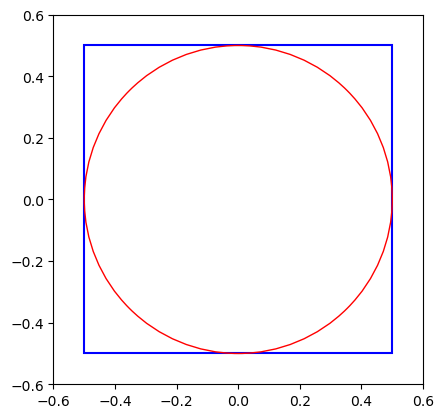
\includegraphics[width=0.6\textwidth]{../resources/motivation/inscribed_circle.png}
    \end{figure}
\end{frame}

\begin{frame}{Гиперсфера и гиперкуб}
    \begin{itemize}
        \item Объем гиперсферы стремится к нулю при росте размерности:
              \begin{equation*}
                  V_n = \frac{\pi^{n/2}}{\Gamma(\frac{n}{2}+1)}R^n
              \end{equation*}
        \item Диагональ гиперкуба увеличивается как \(\sqrt{n}\).
    \end{itemize}
    \begin{figure}
        \centering
        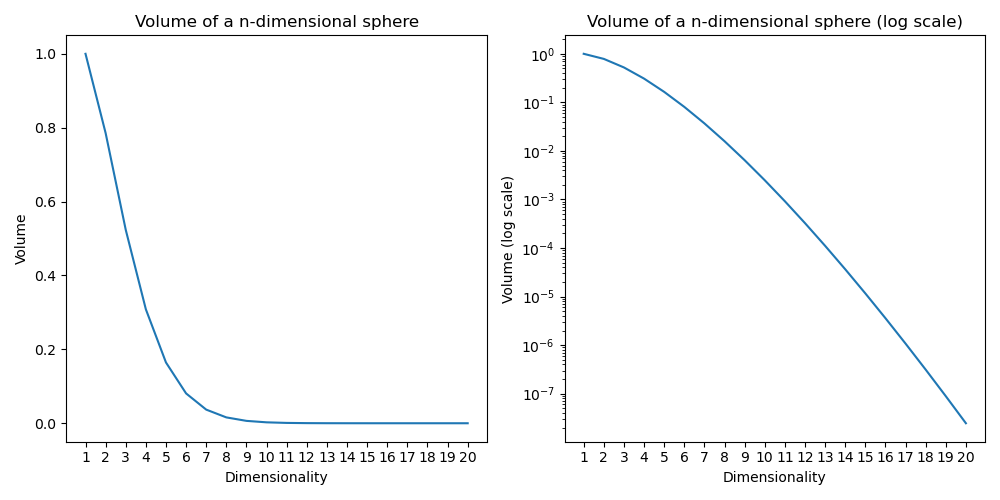
\includegraphics[width=0.7\textwidth]{../resources/motivation/sphere_volume.png}
    \end{figure}
\end{frame}

\begin{frame}[allowframebreaks]{Влияние на метрические модели}
    \begin{itemize}
        \item Манхэттенское расстояние:
              \begin{equation*}
                  d(x^{(i)}, x^{(j)}) = \sum_{k=1}^n |x_k^{(i)} - x_k^{(j)}|
              \end{equation*}
        \item Средние расстояния между точками становятся близкими:
              \begin{equation*}
                  \lim_{n\to\infty}\frac{d(x^{(i)}, x^{(j)})}{n} = \mu
              \end{equation*}
        \item Сохраняется и для $L_2$ нормы.
    \end{itemize}
    
    \begin{figure}
        \centering
        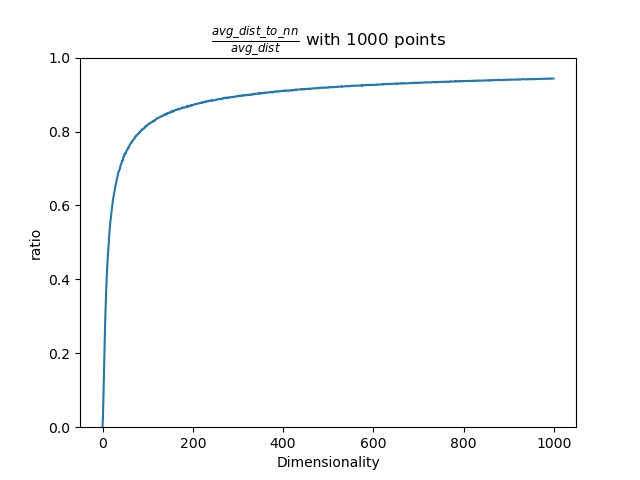
\includegraphics[width=.7\textwidth]{../resources/motivation/ratio.png}
    \end{figure}
\end{frame}

\begin{frame}{Линейная регрессия и мультиколлинеарность}
    \begin{itemize}
        \item Решение задачи MSE:
              \begin{equation*}
                  (X^TX)\hat{\beta} = X^Ty
              \end{equation*}
        \item Матричная ковариация:
              \begin{equation*}
                  \mathrm{Cov}(X) = \frac{1}{k-1}X^TX
              \end{equation*}
        \item Высокая корреляция между признаками \(\Rightarrow\) нестабильные веса, переобучение.
    \end{itemize}
\end{frame}

\begin{frame}{Влияние на "деревянные" модели}
    \begin{itemize}
        \item Сложность выбора оптимального разделения при высокой размерности.
        \item Деревья склонны к переобучению из-за случайных разбиений.
        \item \textbf{Workaround:} \textit{Random Subspace Method} (Но)
    \end{itemize}
\end{frame}

\begin{frame}{Влияние на глубокие нейронные сети}
    \begin{itemize}
        \item Сверточные сети (\textit{CNN}) используют локальные взаимосвязи.
        \item \textit{LSTM} моделируют временные зависимости, игнорируя пространственные.
        \item Трансформеры извлекают только значимые зависимости.
        \item Проблемы: обучение на шуме, сложность оптимизации функционала потерь.
    \end{itemize}
\end{frame}

\begin{frame}{Общее влияние "проклятия размерности"}
    \begin{itemize}
        \item Увеличение времени обучения моделей.
        \item Сложность интерпретации табличных данных.
        \item Вероятность обучения на шумовых признаках \(\Rightarrow\) переобучение.
    \end{itemize}
\end{frame}